\documentclass[12pt]{article}
\usepackage[english]{babel}
\usepackage[utf8x]{inputenc}
\usepackage[T1]{fontenc}
\usepackage{lab}
\usepackage{listings}
\usepackage{comment}


\Instructors{Alex Mussa, Kevin Johnson}
\LabNumber{2}
\LabTitle{Electronic Components and Lab Equipment}
\LabDate{June 26th, 2019}

\lstset{style=mystyle}

\begin{document}
\MakeLabTop

\section{Introduction}

In the lab, you will find equipment such as oscilloscopes, waveform generators, multimeters, power supplies, cables, circuit components, and a desktop computer with useful softwares that will all aid in the design, analysis, and prototyping of circuits. Lab equipment is useful for many tasks, such as using in experiments to validate basic theoretical representations of electricity or testing your robots new designs changes. In these lab 2 exercises, we will focus on experimenting with and understanding the basic concepts of electricity, and becoming familiar with the equipment available and how to operate it. We will continue progressing towards understanding how, in an electrical sense, the various components of the Tumbller self-balancing robot work together, so you can interface some new circuit elements with it successfully later in the semester. 

\section{Setup}

\subsection{Gathering additional materials from instructors}

You will need to have a sensor kit as well as a breadboard and wire kit in order to complete the lab assignments. Make sure you have the sensor kit, a breadboard, and jumper wires. If you do not, ask the instructor for whatever you are missing. The sensor kit contains 37 various circuit elements such as sensors on small printed circuit boards as well as some resistors. Although this kit will be primarily used with the Tumbller robot, some of the sensors and resistors will be used for testing in the lab.


\subsection{Collecting cables for the equipment}

All of the equipment you find at your lab bench needs cables in order for that machine to interface with any circuit you build or want to test. These cable do not come attached to the machines and should not be left attached to the machines. All of the cables available in the lab for the equipment can be found hanging along the walls of the lab. There is a labeled rack of wall hanging cables, which should look like the one displayed in \textit{Figure 1}.

\begin{figure}[H]
    \centering
    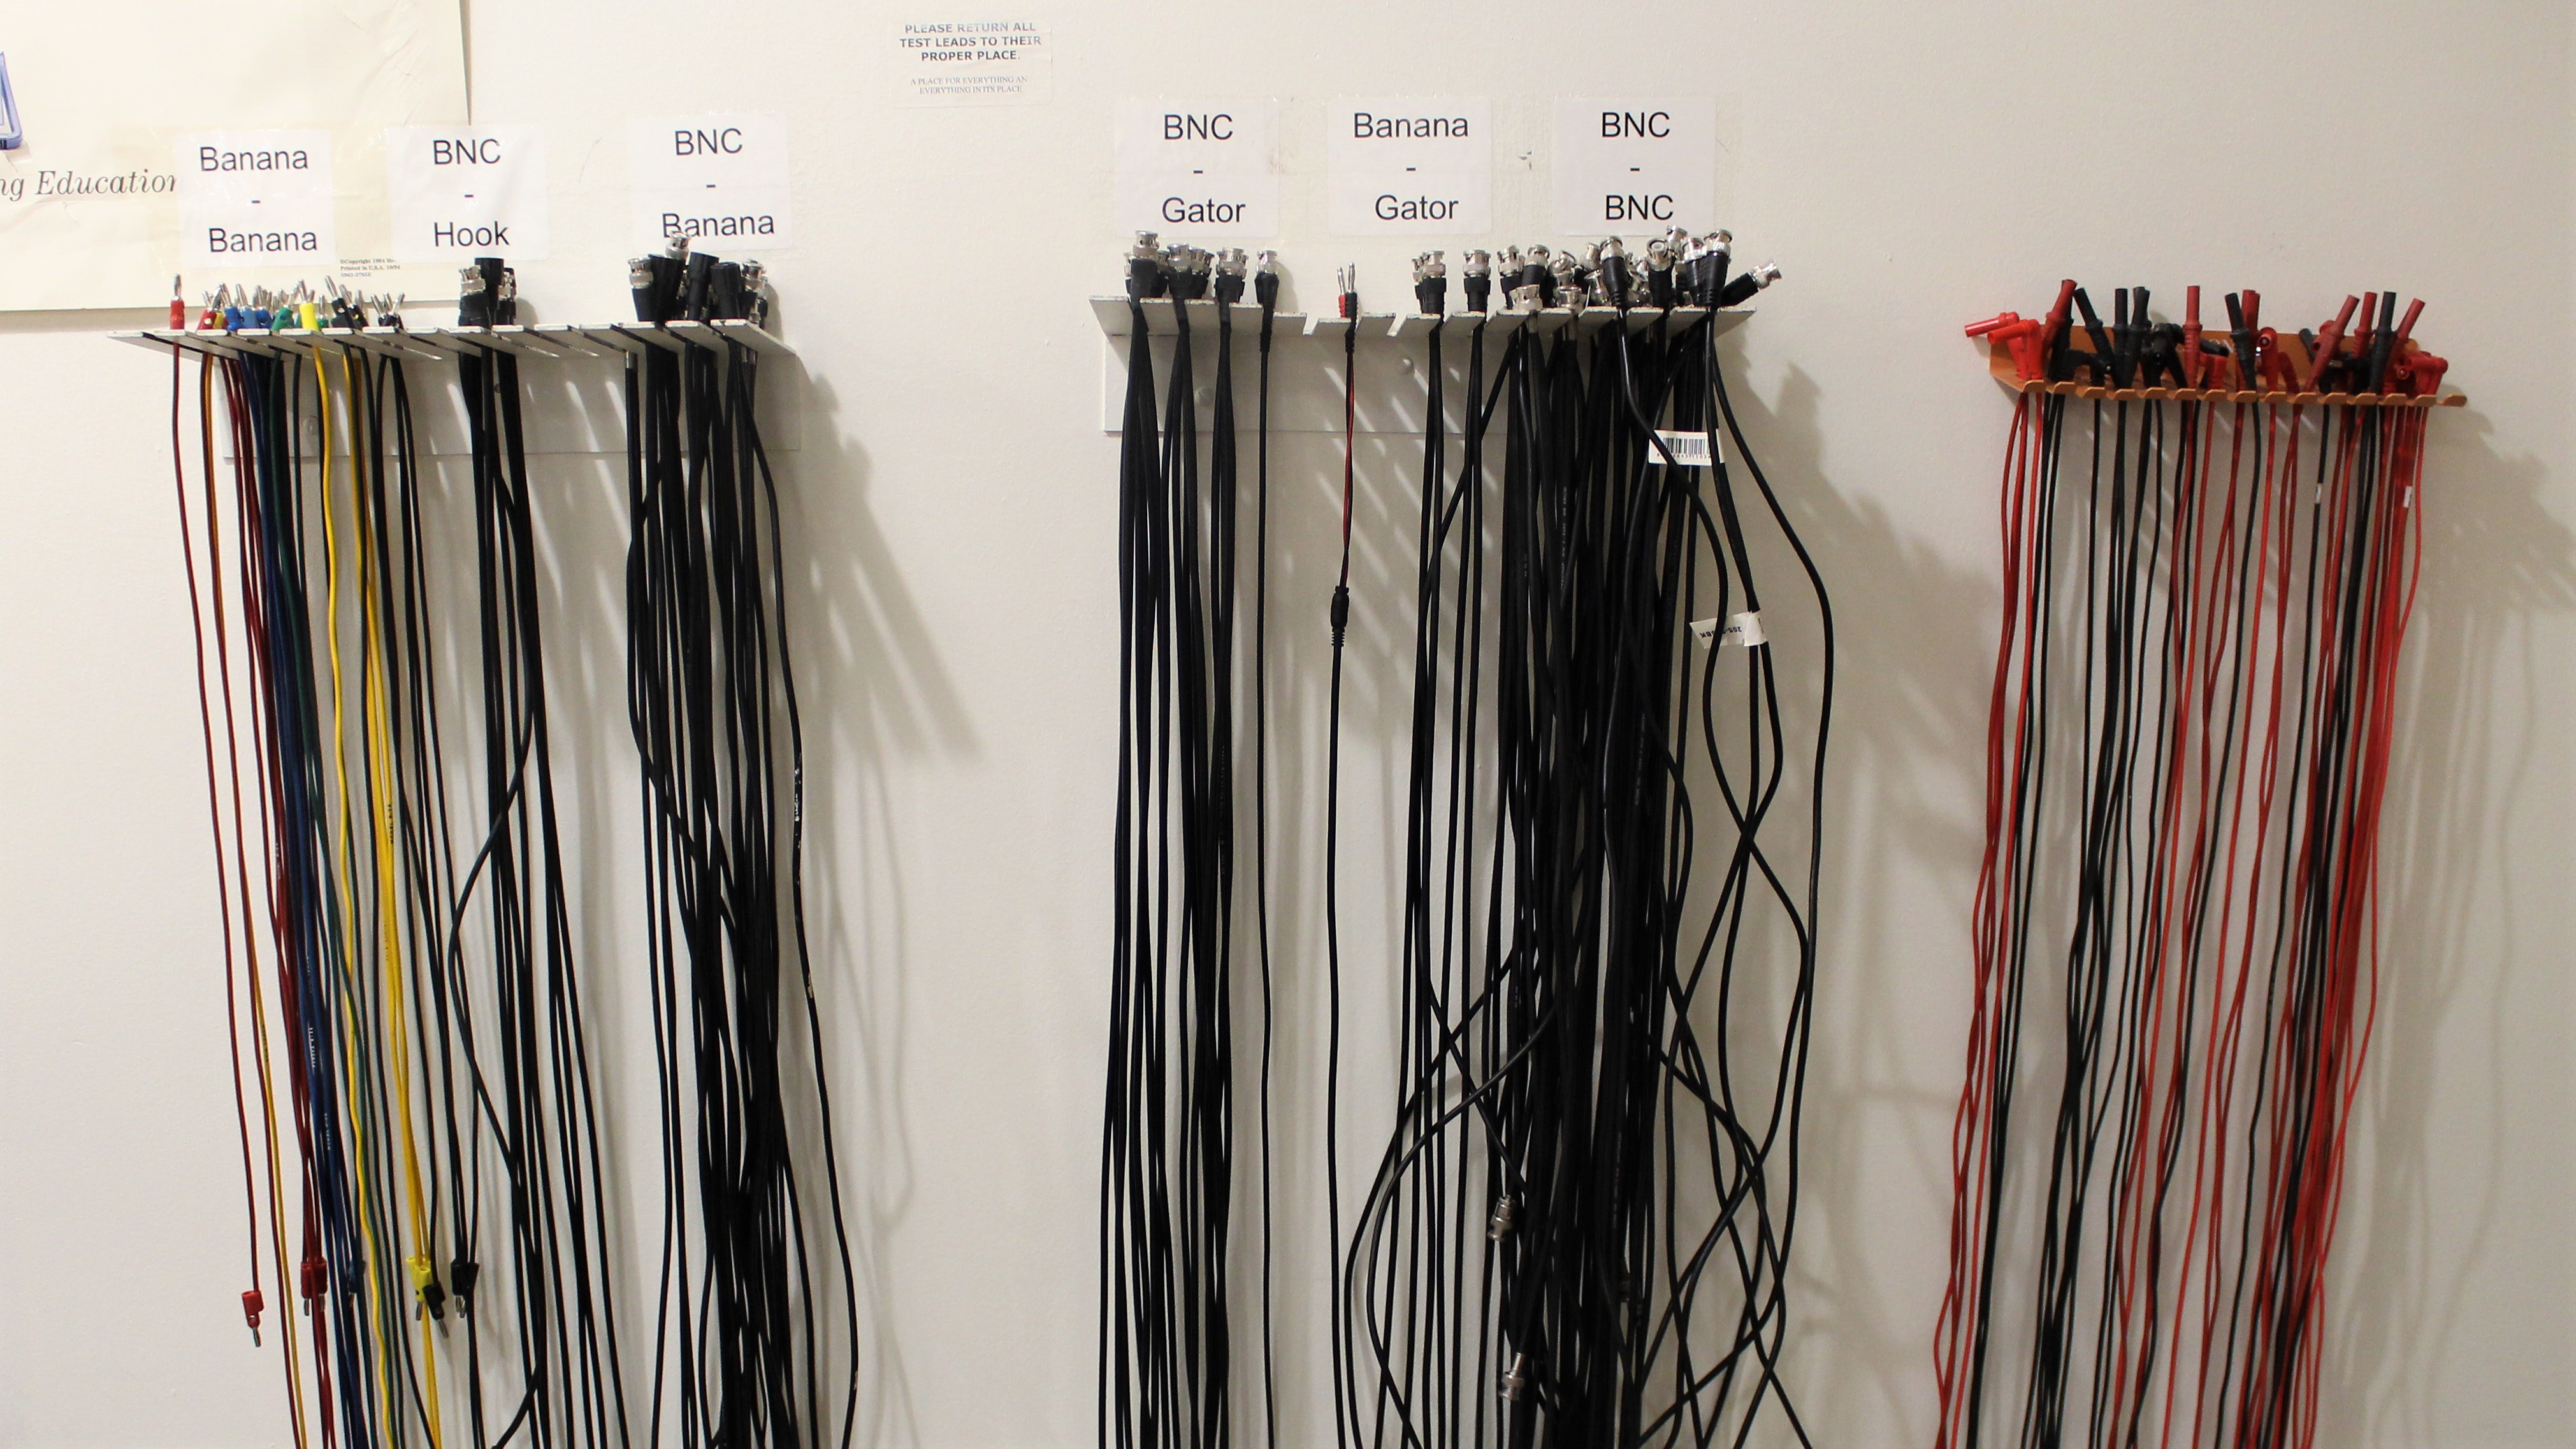
\includegraphics[width=15cm]{photos/lab/wallcables.jpg}
    \caption{Wall hanging cables found in the lab.}
\end{figure}

\textbf{\underline{INSTRUCTIONS}}

\begin{enumerate}
    \item Locate the wall hanging rack in the lab room.
    \item Gather the following cables: 
    \begin{enumerate}
        \item 1 \textit{Banana-to-alligator cable}
        \item 2 \textit{BNC-to-alligator cable}
        \item 1 \textit{Red DMM cable (banana-to-probe; unlabeled in figure)} 
        \item 1 \textit{Black DMM cable (banana-to-probe; unlabeled in figure)}
    \end{enumerate}
    \item Connect the banana connector side of the Banana-Gator cable to the DC power supply. Do not power on the power supply.
    \item Connect the BNC connector side of one of the BNC-Gator cables to the first channel of the Oscilloscope. Do not power on the oscilloscope.
    \item Connect the BNC connector side of one of the BNC-Gator cables to the first channel of the Arbitrary Waveform Generator. Do not power on the wave gen.
    \item Connect the circular end of the red DMM cable into the red port on the front panel with the $\Omega$ symbol. Connect the black DMM cable to the rightmost black port on the front panel with the LO imprint. Turn the power switch to the on  position on the leftmost side of the front panel of the DMM.
\end{enumerate}

\section{Experiments}
\subsection{Calculating and Measuring Resistance of Resistors}

The through-hole resistors found in the bottom right side of the sensor kit come in a variety of resistance values. Although the resistors have specifications printed on the package, they also have a color code on their bodies which represents the resistance. One of the color bands indicates the tolerance of the resistor as a percentage, representing the range of variability of the actual resistance of the resistor from its labeled rating. As such, the actual resistance of the resistor will likely vary from its rating slightly. Thus, in order to understand exactly how much resistance the material within the physical resistor introduces to a circuit, a measurement with a multimeter is necessary.

Take the resistors out of your sensor kit and grab one of each of the resistor values listed below in \textit{Table 1}. Then, with the lab bench digital multimeter turned on, press the blue \texttt{SHIFT} button and then  press the button labelled $\Omega 2W$. The DMM is now ready to take measurements of resistors. To take a measurement of a resistor, press the red probe to one end of the resistor and the black probe to the other.  Do not hold the wires in your hands, or you will measure the resistor in parallel with the resistance of your body.  Allow time for the DMM to take then measurement and then read the resistance value from the display of the DMM. Do this for each of the resistors collected and record the measured resistance into \textit{Table 1}. Then, compute the difference between the measured and rated resistance, as well as the percentage variation from the rated value.

\begin{table}[H]
    \centering
    \begin{tabular}{|c||l|l|l|}
        \hline
        Rated Resistance & Measured Resistance & $(Measured - Rated)$ & $\frac{(Measured - Rated)}{Rated}$  \\ \hline \hline
        $220\Omega$      &                     &                      &                                     \\ \hline
        $330\Omega$      &                     &                      &                                     \\ \hline
        $1k\Omega$       &                     &                      &                                     \\ \hline
        $5.1k\Omega$     &                     &                      &                                     \\ \hline
        $100k\Omega$     &                     &                      &                                     \\ \hline
        $1M\Omega$       &                     &                      &                                     \\ \hline
    \end{tabular}
    \caption{}
\end{table}

When you have finished taking the measurements and computing the values for \textit{Table 1}, answer the questions below.
\newpage
\textbf{\underline{QUESTIONS}}
\begin{enumerate}
    
    \item The resistors provided in the sensor kit all have a 1\% tolerance rating. Compare the values computed in column 4 to the expected 1\%. Are they within an acceptable range? What do you notice about the values in column 3 (absolute error) as the resistances get larger? 
        \fillwithlines{1in}
        
    \item Thinking of each individual resistor as a unique set of materials, why do you think the resistors you measured have resistance values different from that of the nominal value? Considering two resistors of the same rating, why do you think two resistors of the same specification could have different resistances?
        \fillwithlines{1in}
        
    \item Observe the third and fourth columns of \textit{Table 1} (absolute error and percentage error). In what situations do you think these values are important? That is, what might a variation in resistance change in a circuit and why do you think this may be important to know?
        \fillwithlines{0.8in}

% Haven't discussed power in lecture yet
\begin{comment}
    \item One thing to be aware of when using resistors is the power rating of the resistor you are using. If the resistor exceeds the amount of power it is rated for, the amount of heat dissipation is too much for the material to handle and can cause the material to start burning. If the $220\Omega$ resistor is rated at $\frac{1}{4}W$, what is the highest value of voltage that can be applied to keep the power within the resistors power rating of $\frac{1}{4}W$? HINT: Use ohm law and the power equation to solve for the voltage when $P=\frac{1}{4}W$.
        \framebox(439,100){}
\end{comment}

\end{enumerate}         

Using a digital multimeter is very convenient to measure the actual resistance with the resistance setting. However, it is also possible to compute the resistance of the resistor by applying some known voltage across it and measuring the current. With this information, the resistance can be computed with Ohm's law. In order to perform this experiment, you will need to build the following circuit, shown in \textit{Figure 2}.

\begin{figure}[H]
    \centering
    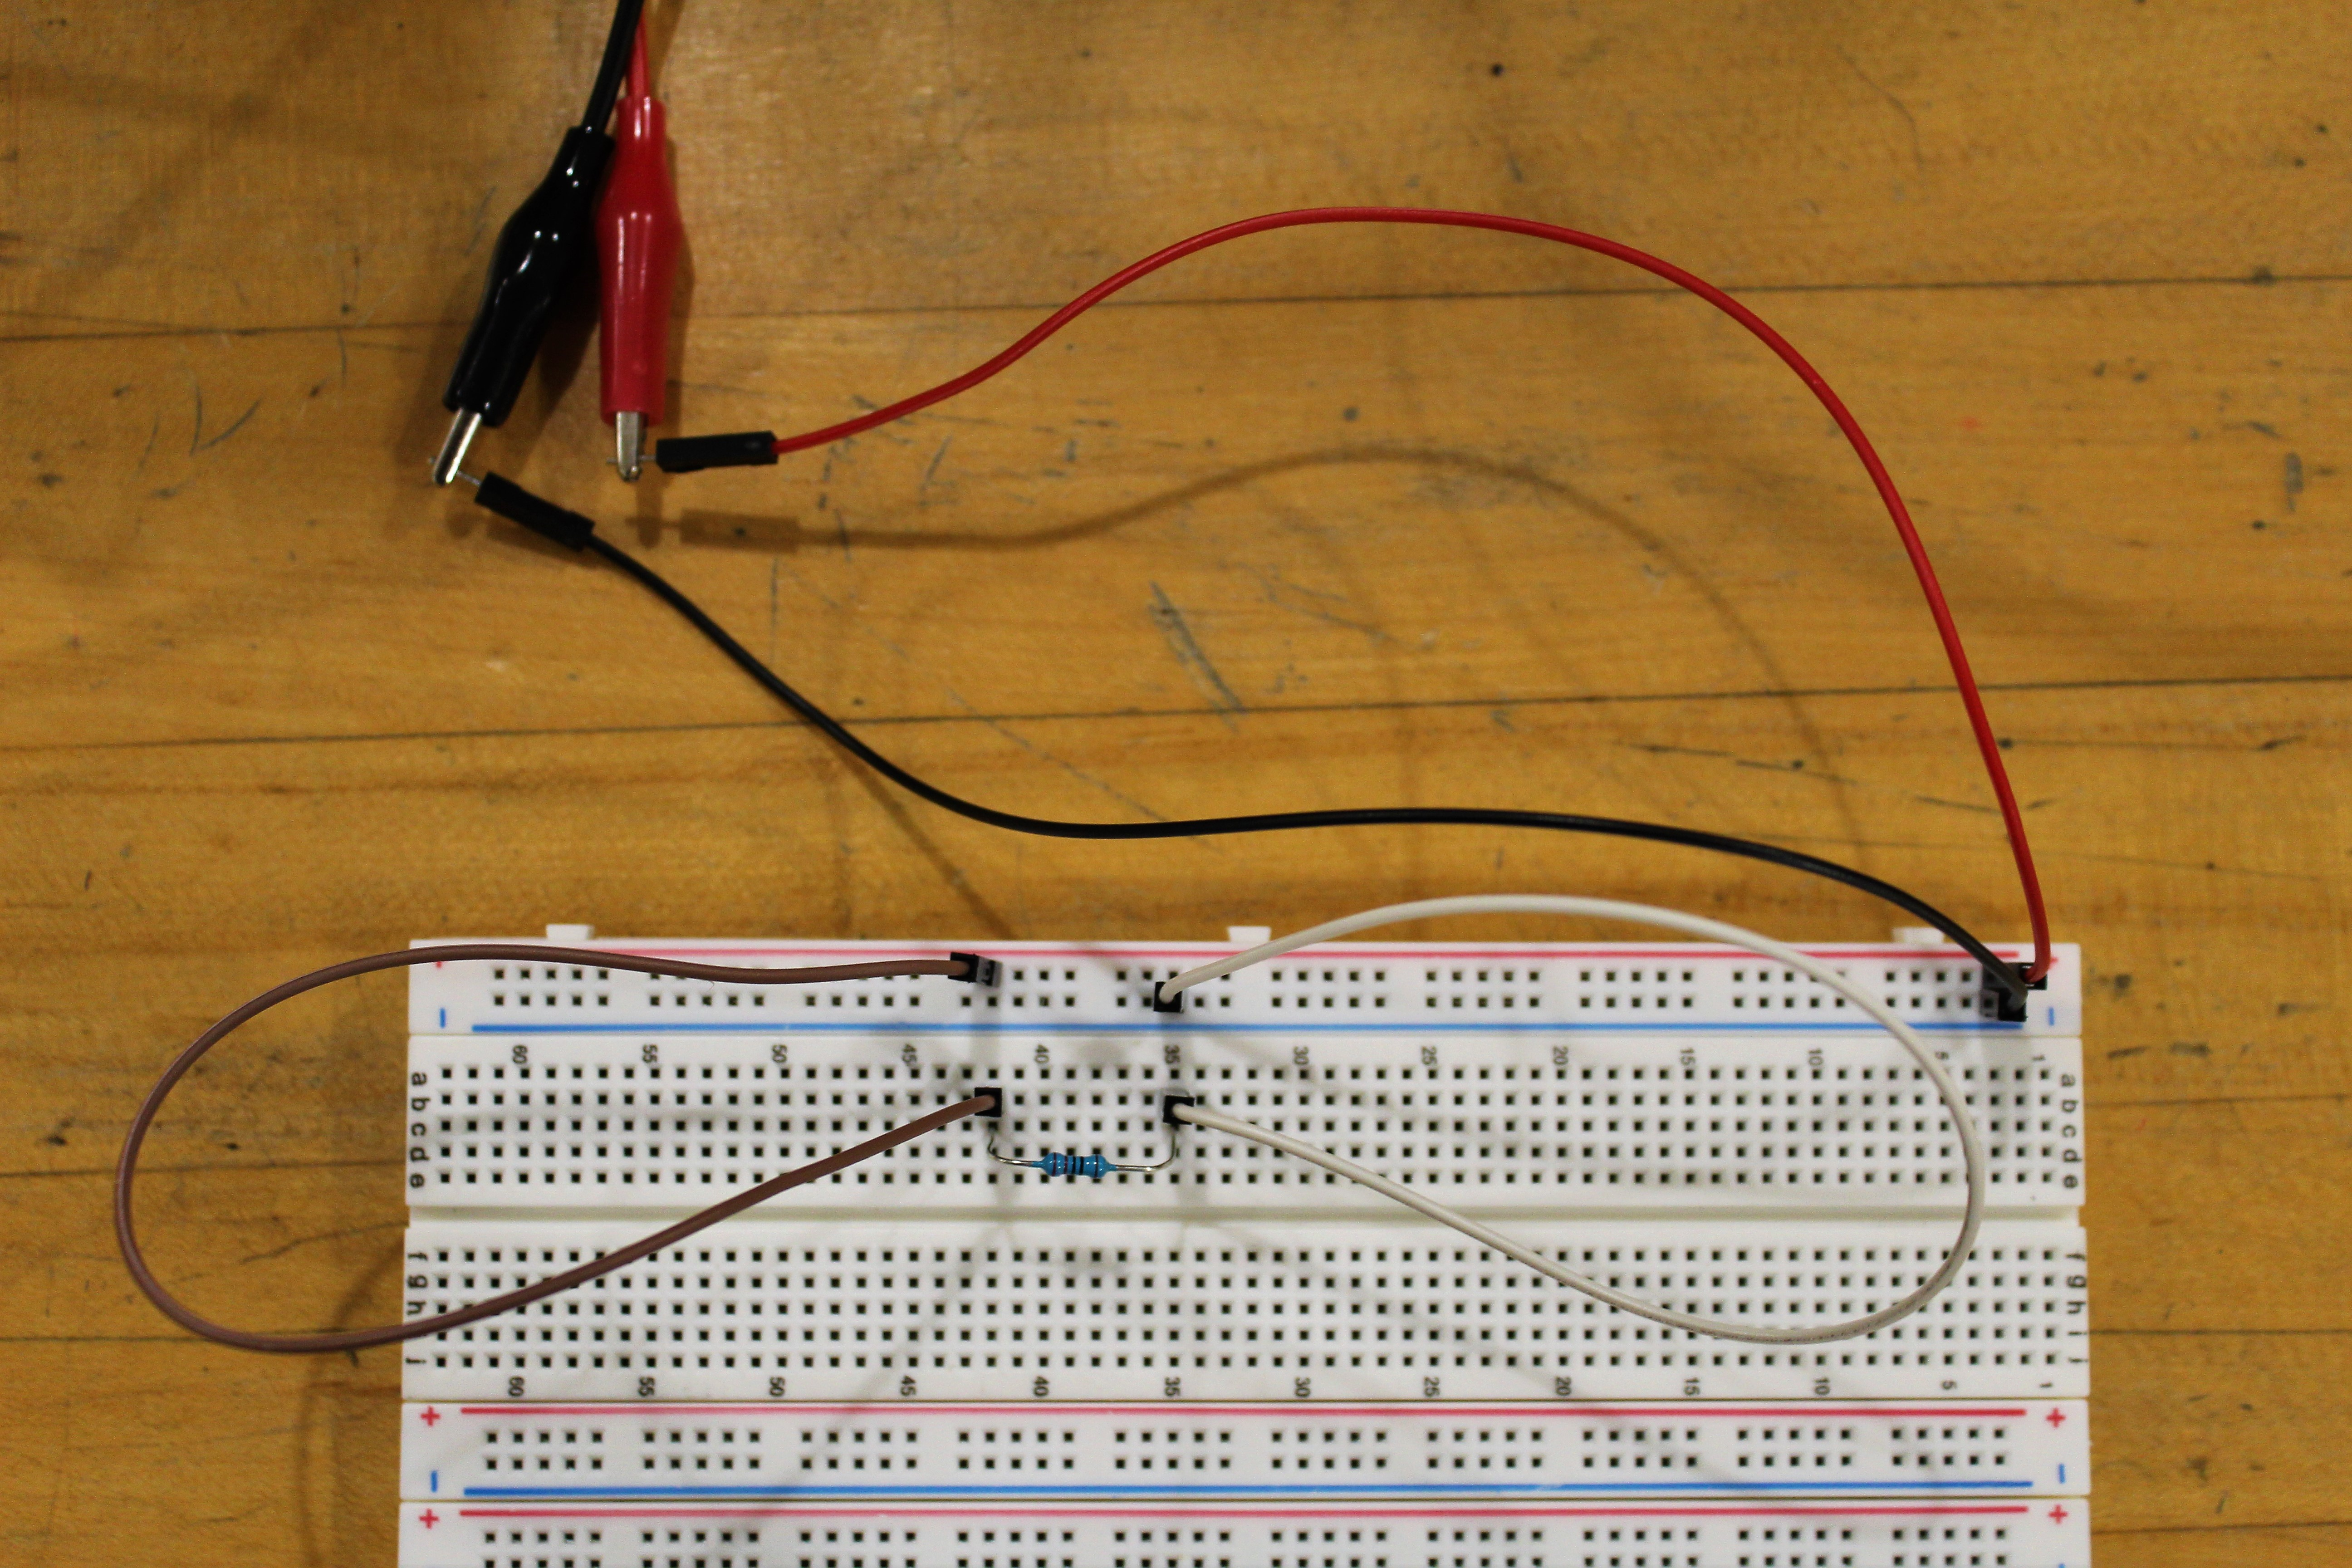
\includegraphics[width=12cm]{photos/lab/resistorcircuit.jpg}
    \caption{An example of a resistor connected to a power supply with wires on a breadboard.}
\end{figure}

\textbf{\underline{INSTRUCTIONS}}
\begin{itemize}
    \item Confirm that the power supply is off, and turn the +6V adjustment knob to 0 (fully counter-clockwise).
    \item Starting with $220\Omega$, construct the circuit in \textit{Figure 2}.
    \item Ensure that the power supply's built-in multimeter is set to measure the +6V output by pressing the +6V button under the meter. Turn on the supply and adjust the output voltage to approximately 2V.  The meter on the power supply should indicate that current is flowing, and since the only component connected is a resistor, that voltage and current could be used to calculate resistance.  However, that cannot be used for elements in more complicated circuits, so you will generally need to use the multimeter to measure voltage and current.
    \item On the multimeter, press the \texttt{DC V} button under function to switch it to measuring DC voltage, and ensure that the red probe is inserted in the voltage input.  Use the multimeter to measure the voltage across the resistor, and record the voltage in \textit{Table 2} below.
    \item T measure the current flowing through the resistor with the same multimeter, first change the red lead (wire) to the bottom red input terminal labeled with a red I (which stands for current). Then, under functions, select \texttt{SHIFT} and \texttt{DC I}. Remember that you must break the circuit and insert the multimeter in order to measure the current. Record the current in the table below.  WARNING: when finished measuring current, ALWAYS move the probe back to the voltage input (or simply remove it entirely).  Leaving the probe in the current input will inevitably lead to someone blowing a fuse when they try to use the DMM to measure voltage.
    \item Repeat this procedure for all of the resistors. When finished, compute the resistance and record in the below table.
\end{itemize}

\begin{table}[H]
    \centering
    \begin{tabular}{|c||l|l|l|}
        \hline
        Rated Resistance & Measured Voltage & Measured Current & Calculated Resistance  \\ \hline \hline
        $220\Omega$      &                  &                  &                        \\ \hline
        $330\Omega$      &                  &                  &                        \\ \hline
        $1k\Omega$       &                  &                  &                        \\ \hline
        $5.1k\Omega$     &                  &                  &                        \\ \hline
        $100k\Omega$     &                  &                  &                        \\ \hline
        $1M\Omega$       &                  &                  &                        \\ \hline
    \end{tabular}
    \caption{}
\end{table}

When you have finished taking the measurements and computing the values for \textit{Table 2}, answer the questions below.

\textbf{\underline{QUESTIONS}}
\begin{enumerate}
    \item Compare the calculated resistance in \textit{Table 2} with the measured resistance from \textit{Table 1}. How do they compare? Is this expected? Why or why not?
        \fillwithlines{1in}
    
    \item If you utilized the power rails in your circuits build such as the figure did, could you have not? If so, how would it be done? When would it be beneficial to use the power rails?
        \fillwithlines{1in}
\end{enumerate}

\checkoffsubsub

\subsection{Using the Oscilloscope and Waveform Generator}

In some cases, it may be necessary to view a plot of how voltage changes over time. This is especially true for alternating waveforms, such as those produced by the waveform generator. Whereas a DC power supply generates a signal that only varies in voltage if the setting is changed, waveform generators make signals with voltage that varies periodically over time. These waveforms are generated according specified parameters, such as frequency, amplitude, and shape, which dictate the behavior of the signal. In order to determine if a circuit that utilizes such signals is behaving appropriately or to get a better understanding of what is happening at a particular point within a circuit, an oscilloscope can be used.

\begin{figure}[H]
    \centering
    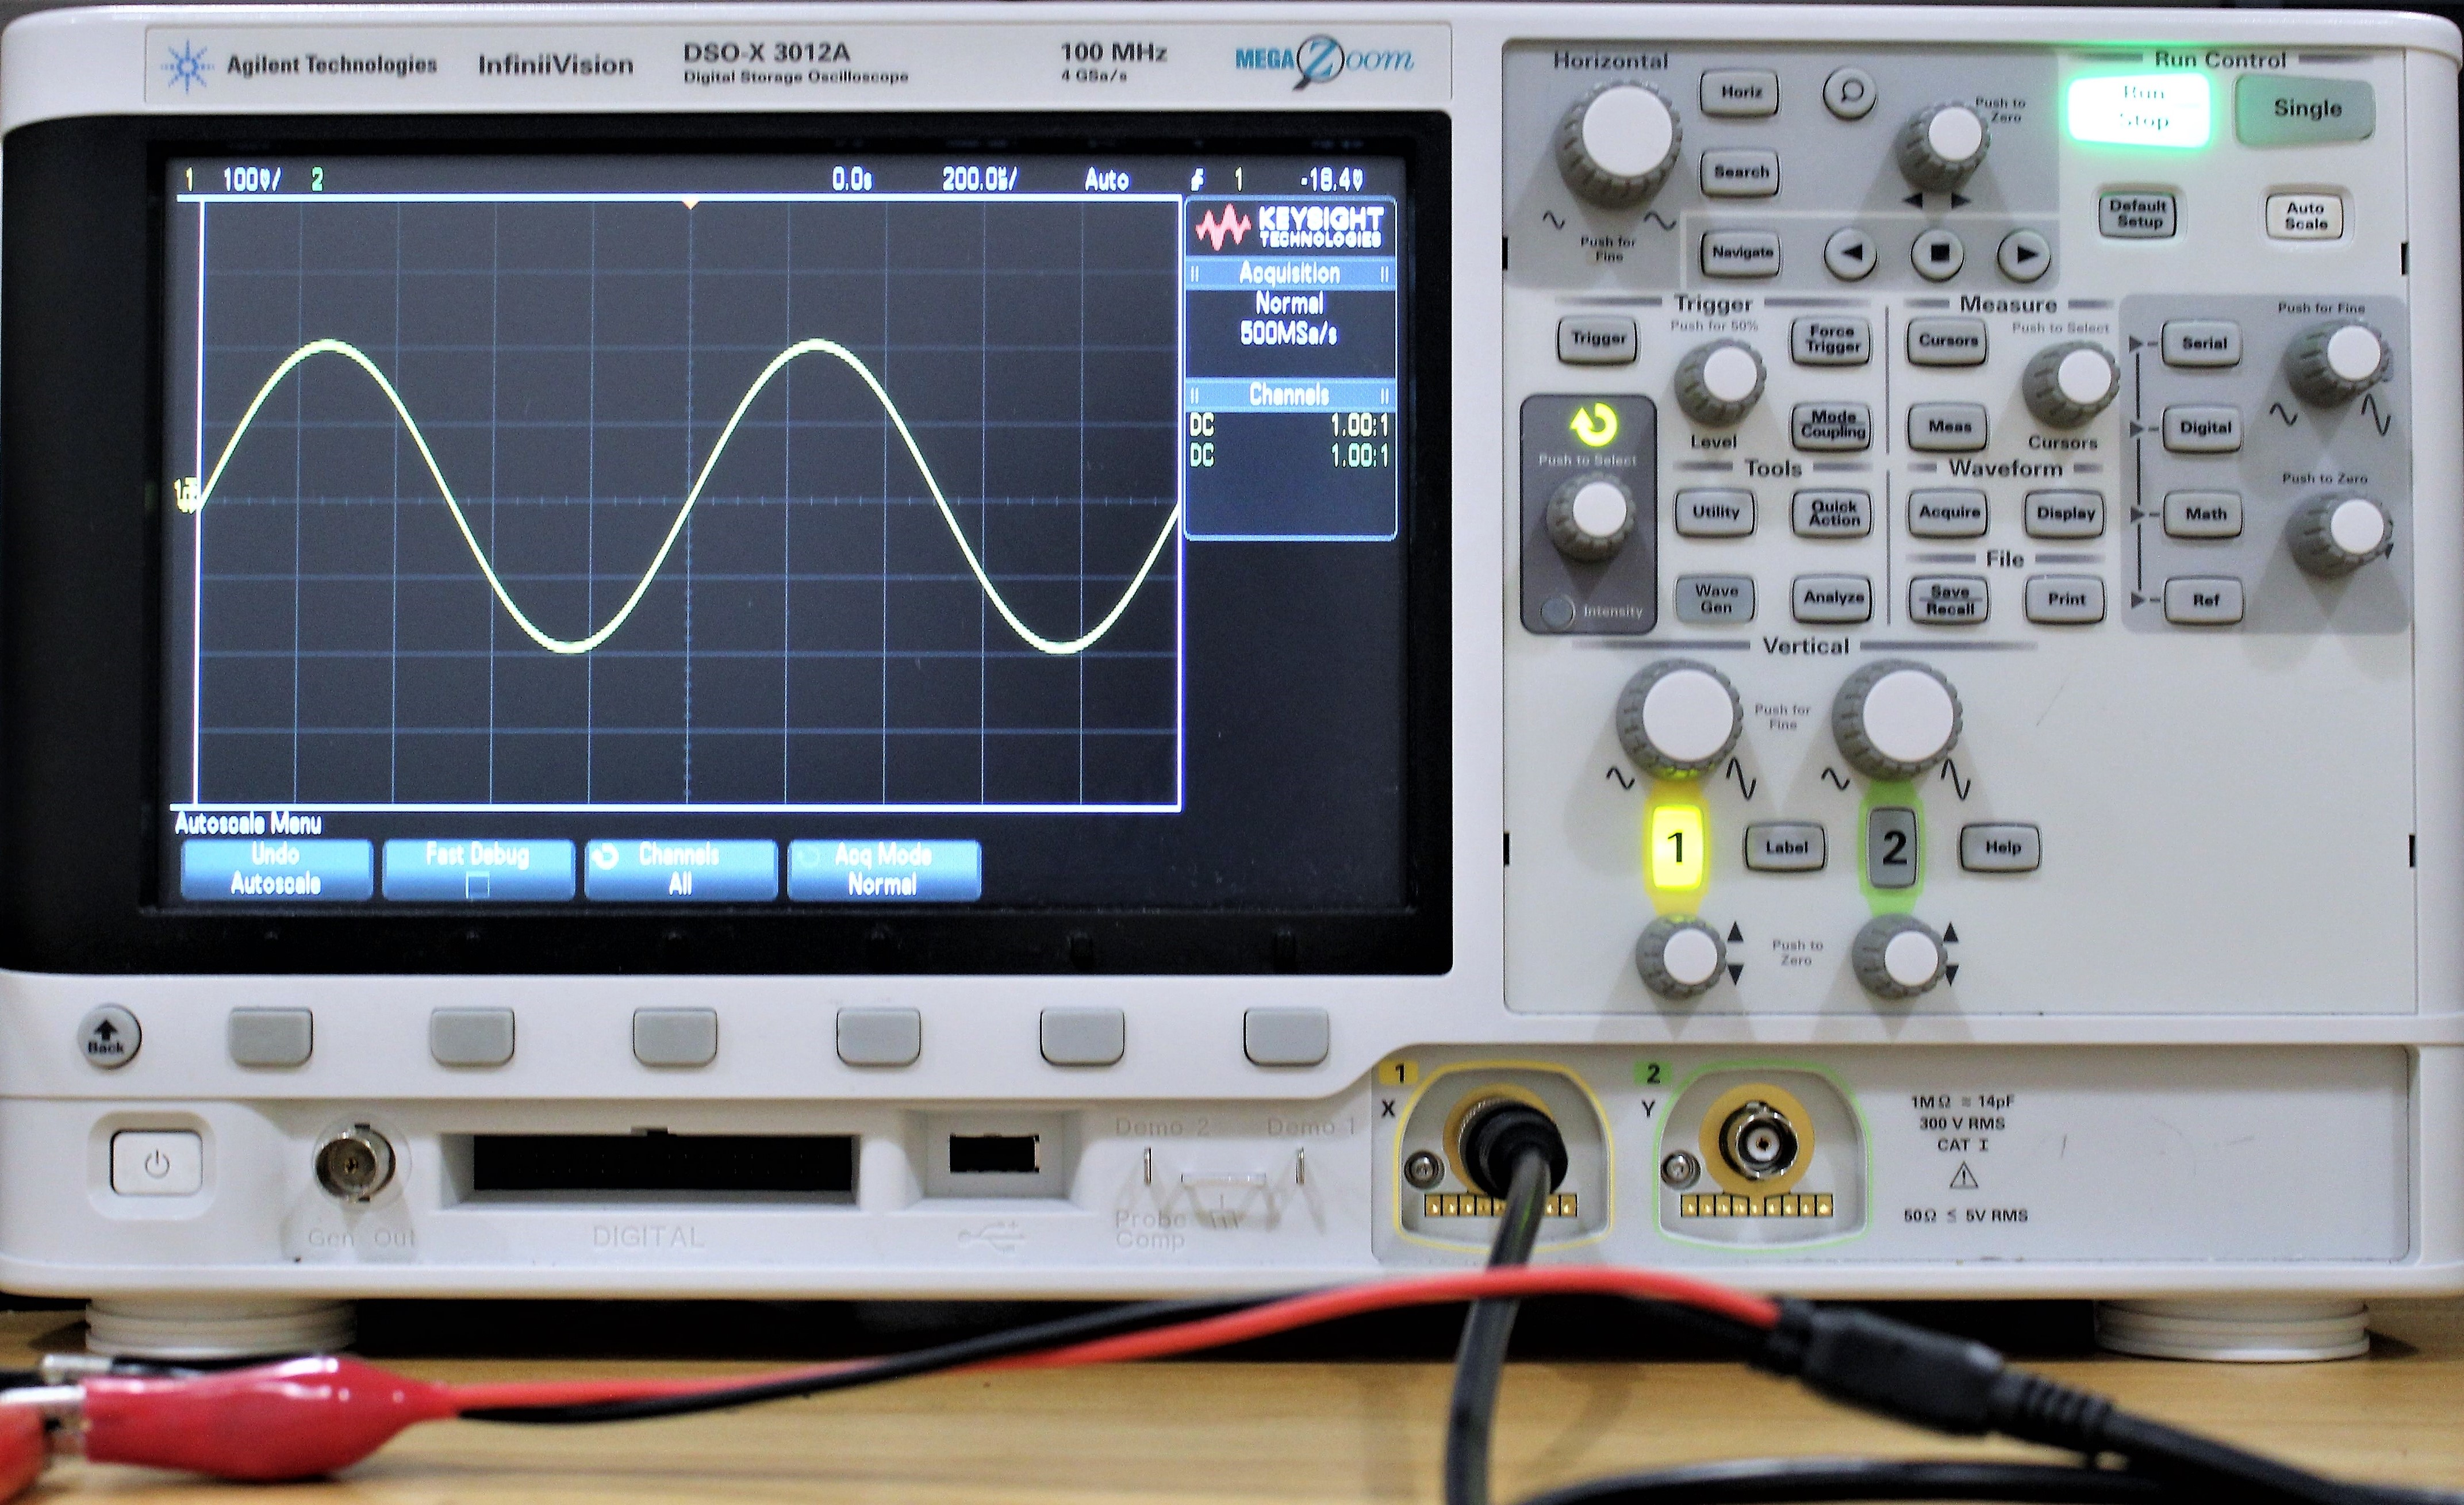
\includegraphics[width=12cm]{photos/prelim/oscilloscope.jpg}
    \caption{An oscilloscope connected directly to a waveform generator producing a 1kHz $400mV_{pp}$ sine wave.}
\end{figure}

Before beginning the experiment, answer the following question. When you are finished answering the question, proceed to the experiments instructions.

\textbf{\underline{QUESTION}}
\begin{enumerate}
    \item Observe the oscilloscope's display in \textit{Figure 3}. The peak-to-peak amplitude of the wave was computed as an example in the preliminary reading materials. In a similar fashion, compute the frequency by finding the period, T, in seconds and using the formula for frequency, $f = \frac{1}{T} Hz$. Note that there are two cycles of the waveform displayed on the screen and the period is calculated from just one.
    
    \framebox(439,100){}
\end{enumerate}
\newpage
\textbf{\underline{INSTRUCTIONS}}

\begin{enumerate}
    \item Connect the red alligator clip of the BNC-to-alligator cable connected to you waveform generator to the red gator clip of the BNC-to-alligator cable connected to your oscilloscope. Repeat for the black alligator clips of the two cables.
    \item Turn the power on for both the oscilloscope and waveform generator. Note that the waveform generator will not output a signal until you enable the output.
    \item On the waveform generator, select the oval \texttt{Waveforms} button. Read through the available waveforms and find the Sine wave, and select it by pressing the button under the label.
    \item Select the rectangular \texttt{Parameters} button. For this waveform, choose an Amplitude of $1V_{pp}$, a frequency of $10 Hz$, offset of 0, and phase of $0^{\circ}$.
    \item Turn on the output of the waveform generator by selecting the button labeled "1" above the BNC output and then selecting \texttt{Output: ON}.
    \item The waveform should now be present at the oscilloscope input, but the scaling on the oscilloscope may be off. Start by using the \texttt{AUTOSCALE} feature on the oscilloscope to get a reasonable scaling, and then use the knobs located under the \texttt{HORIZONTAL} and \texttt{VERTICAL} labels to adjust the time (horizontal) scaling so there are two cycles of the signal present on the screen and the amplitude (vertical) resolution such that the top of the waveform touches the top most grid line and the bottom of the waveform touches the bottom most grid line.
\end{enumerate}

When you have finished, record the final values of your adjusted resolution in the lines below.
\begin{center}
    Vertical Scaling:   \underline{\hspace{4cm}} /div
    
    Horizontal Scaling: \underline{\hspace{4cm}} /div
\end{center}

When you are finished recording the values, answer the following questions.

\textbf{\underline{QUESTION}}
\begin{enumerate}
    \item  In the below provided area, sketch the waveform, labeling the time (x-axis) fully as well as the amplitude (y-axis). Label the frequency of the waveform, the period, and the peak-to-peak voltage.
    
    \framebox(439,300){}
\end{enumerate}

Continue following through the instructions and complete the experiment.

\textbf{\underline{INSTRUCTIONS}}

\begin{enumerate}
    \item Now change the frequency of the sine wave from $10 Hz$ to $1kHz$. 
    \item Press the \texttt{AUTOSCALE} button on the oscilloscope and not the scaling change.
    \item On the oscilloscope, select the \texttt{Meas} button under the \texttt{Measure} section of the oscilloscope. A menu called \texttt{Measurement Menu} should populate on the bottom of the oscilloscopes display. Make sure the source is selected to channel 1, as this is the channel the waveform is coming in on. To do this, select \texttt{Source} in the measurement menu with the buttons under the display and select 1 with the selection knob located right the display within the dark grey boxed area containing the illuminated green circular arrow.
    \item In the measurement menu, select the \texttt{Type:} option and scroll through the menu and find frequency. When you have higlighted \texttt{Freq}, click the knob to select it.
    \item When you are finished selecting the measurement, select the \texttt{Add Measurement} option from within the measurement menu. This will add the measurement of frequency to the right side of the display under \texttt{Measurements}.
    \item Add a second measurement of the peak to peak voltage by following through the same step, but selecting the peak to peak voltage as the desired measurement.
    \item When both the peak to peak voltage and the frequency are displayed on the screen, record the values below.
    
    \begin{center}
    Frequency   \underline{\hspace{2cm}} Hz
    
   Peak-to-Peak Voltage: \underline{\hspace{2cm}} V
\end{center}
\end{enumerate}

\textbf{\underline{QUESTIONS}}
\begin{enumerate}
    \item Having computed the peak-to-peak voltage and frequency both manually and automatically, hypothesize how the oscilloscope might be computing the frequency and peak to peak voltage given the signal's voltage values being stored into memory. How do you think the oscilloscope is computing these values? Think of how you computed the values manually.
        \fillwithlines{1in}
    
    \item If the sine wave depicted in \textit{Figure 3} with frequency 1kHz and peak-to-peak amplitude of 400 mV was placed across a 200$\Omega$ resistor, what would the plot of current over time look like? Sketch it with all appropriate labels in the space below.
    
        \framebox(439,300){}
\end{enumerate}

\checkoffsubsub

\subsection{Parallel and Series Resistances}

Recall the below images from the preliminary reading materials. In the following experiment, you will construct the series and parallel circuits and test them with the lab equipment. When you are finished, answer the questions and ask the instructor for a check off.

\begin{figure}[H]
\begin{subfigure}{.5\textwidth}
    \centering
    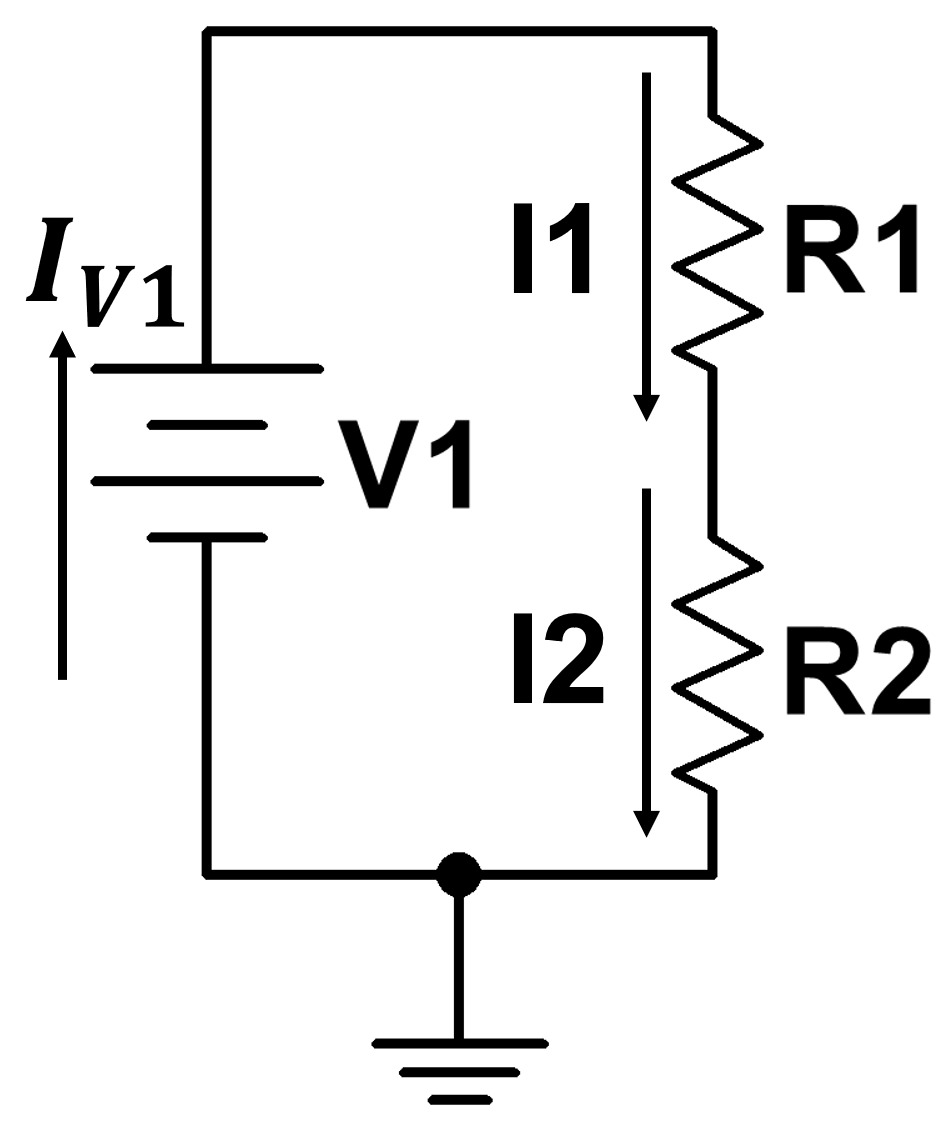
\includegraphics[width=0.7\linewidth]{photos/lab/series.PNG}
    \caption{Series resistors.}
\end{subfigure}%
\begin{subfigure}{.5\textwidth}
  \centering
  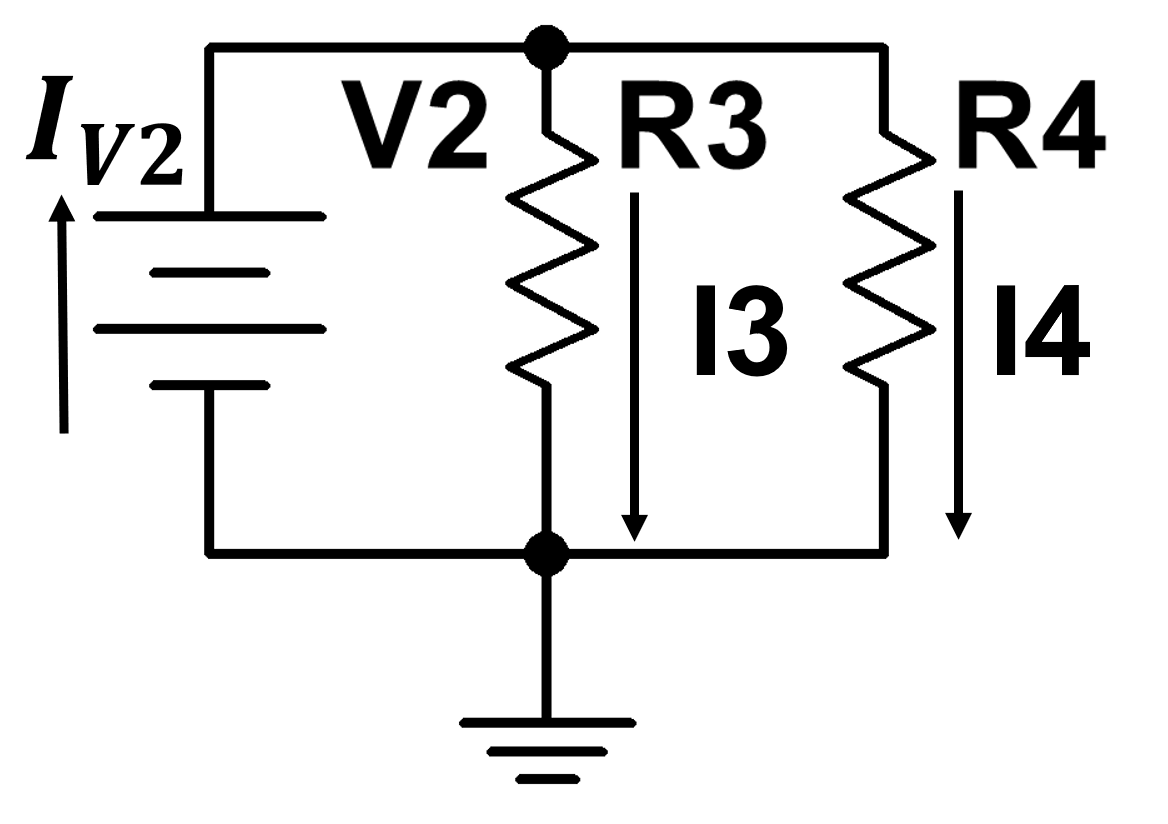
\includegraphics[width=0.8\linewidth]{photos/lab/parallel.PNG}
  \caption{Parallel resistors.}
\end{subfigure}
\caption{Examples of series and parallel resistors in a circuit schematic.}
\end{figure}

From your resistors, grab a $330\Omega$ and $1k\Omega$ and build a series circuit such as the one in the circuit schematic in \textit{Figure 4(a)}. Leave the power supply off while you construct the circuit on the breadboard. Recall that the nodes of a breadboard are internally connected when making these connections. When you are finished constructing the circuit, ensure the voltage of the +6V terminal voltage adjust knob is set to 0 and that the power supply cables are connected correctly. Then, follow the below instructions.

\textbf{\underline{INSTRUCTIONS}}

\begin{enumerate}
    \item Turn the DC power supply on. Adjust the voltage knob to supply 2.7V. 
    \item Use the DMM to measure the voltage across each resistor. Record the values in the \textit{Table 3}.
    \item Now, use the DMM to measure the current through each resistor. Record those values in the \textit{Table 3}.
    \item Turn off the power supply when finished.
    \item Construct the circuit in a parallel configuration such as the one in \textit{Figure 4(b)}. Now, repeat steps 1-4 for the parallel configuration, making sure to record the values in the table and turn off the power supply when finished.
\end{enumerate}

\begin{table}[H]
    \centering
    \begin{tabular}{|c||l|l|l|l|}
        \hline
            & \hspace{0.5cm} $V_{330\Omega}$ \hspace{0.5cm}    & \hspace{0.5cm}  $V_{1k\Omega}$ \hspace{0.5cm}  &   \hspace{0.5cm} $I_{330\Omega}$  \hspace{0.5cm}   & \hspace{0.5cm} $I_{1k\Omega}$  \hspace{0.5cm}   \\ \hline \hline
           Series &                  &                  &              &          \\ \hline
           Parallel &                  &                  &             &           \\ \hline
    \end{tabular}
    \caption{}
\end{table}

When you have completed the above experiment, answer the following questions.


\textbf{\underline{QUESTIONS}}
\begin{enumerate}
    \item Observe the two voltage drops that occurred across the two resistors in each situation. What can be said about the both of them? Is this expected for each of the conditions? Why or why not? Explain with words, mathematically, or both.
        \fillwithlines{1in}
    
    \item What is the voltage of the series circuit at the point in between the two series resistors when compared to ground? When thinking about this, consider that the path the current must take only travels through 1 resistor at this point, $R_{2}$.
        \fillwithlines{0.3in}
        
    \item What it the voltage between the positive terminal of the power supply and the point in between the two series resistors? Consider that the voltage of the positive terminal is approximately 2.7V and the voltage of the point between the resistors is as previously calculated in question 2.
        \fillwithlines{0.3in}
        
    \item For the parallel circuit, compute the total current supplied by the power supply $I_{V2}$. 
        \fillwithlines{0.3in}
        
    \item Compute the total amount of power supplied by the power supply for the series and parallel combinations. Use the equation $P = V_{1} * I_{V1}$ for series and $P = V_{2} * I_{V2}$ for parallel.
       
         \framebox(439,100){}
        
    \item If these circuits were left running for 2.5 hours and the electric company charged you $\$1.00$/Wh, how much would you owe the electric company? HINT: Start by multiplying the power consumption computed in question 5 with the time duration.
       
         \framebox(439,100){}
\end{enumerate}

\checkoffsubsub

\subsection{Other Circuit Elements: LEDs}

Another basic circuit element that is utilized often in the lab is light emitting diodes, or LEDs for short. These diodes are made of semiconductor materials and operate quite differently from the materials found in resistors. Unlike resistors, LEDs' resistance varies depending on the voltage magnitude and direction applied across it. When a voltage drop is present across the LED from the long lead (the positive lead, or anode) to the short lead (the negative lead, called the cathode), the diode is said to be "forward biased", and the LED's effective resistance drops (and the LED lights). Reverse biasing is when the voltage drop is from the negative lead to the positive lead, and results in the LED exhibiting very high resistance and not illuminating. There is much more happening at the material level, but we will only cover the functional behavior in this class.

\begin{figure}[H]
    \centering
    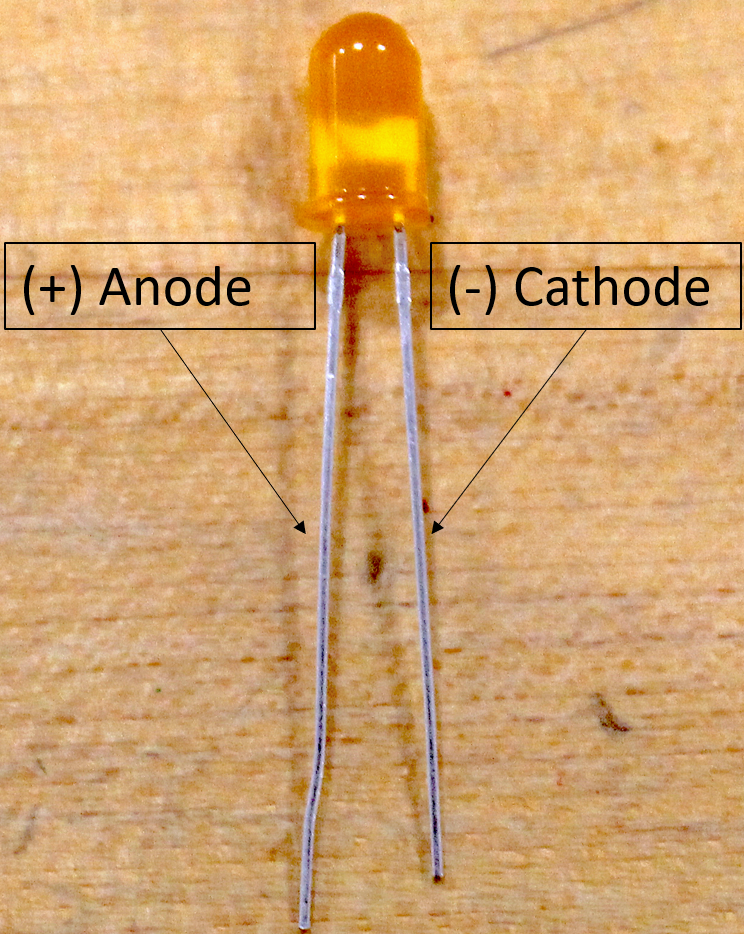
\includegraphics[width=8cm]{photos/lab/led.png}
    \caption{An example of an orange LED.}
\end{figure}

When being forward biased, the LED, being a type of diode, will not permit much current to flow until the LED has reached what is called the \textit{turn on voltage}. At the turn on voltage, the diode is in a state to be able to conduct electrons through the cathode and into the anode. If the applied voltage across the LED is less than this turn on voltage, denoted $V_{TO}$, then the LED will exhibit a higher resistance and thus not conduct enough current to "turn on" or illuminate light.

First start by collecting 2 different color LEDs from the bin. When you have them, record each of their colors at the top of the two tables in \textit{Table 4}. Then, measure their resistance with the DMM by placing the red lead on the anode of the LED and the black on the cathode construct a series circuit such as the one in \textit{Figure 4(a)} where $R_{1} = 220\Omega$ and $R_{2}$ is an LED. The resistor is neccesary in series with the resistor as to limit the amount of current that flows through it as to not overpower the LED. Make sure to leave the power supply off and set the voltage know to zero. Connect the LED into the place of $R_{2}$ such that the long end connects into the same node as $R_{1}$ and the short into ground. When you are finished, continue following the instructions below.

\textbf{\underline{INSTRUCTIONS}}

\begin{enumerate}
    \item Turn on the power supply. Adjust the voltage knob slowly until the LED first turns on. Now, reduce the voltage by exactly 1 volt. Record the voltage and measure the current through the circuit. Record the value in the correct colors table in \textit{Table 4} below.
    \item Calculate the LEDs voltage drop and resistance of the LED, taking into consideration the $220\Omega$ resistor in series. Record the value into the table.
    \item Repeat this process 4 times, increasing the voltage by 0.5 volts every time. This means the third value in the table should be your turn on voltage. Be careful to not look into the LED directly as it passes away from the turn on voltage. Record the voltage and current, and calculate the LED voltage drop and resistance at each step.
    \item When finished with the first LED, repeat for the second.
\end{enumerate}

\begin{table}[H]
    \centering
    LED Color: \underline{\hspace{2cm}}
    
    \begin{tabular}{|l|l|l|l|}
        \hline
            Supplied Voltage & Supplied Current & LED Voltage Drop & Calculated Resistance of LED \\ \hline \hline
            &                  &               &           \\ \hline
            &                  &            &              \\ \hline
            &                  &             &             \\ \hline
            &                  &              &            \\ \hline
            &                  &               &           \\ \hline
    \end{tabular}
    
    LED Color: \underline{\hspace{2cm}}
    
    
    \begin{tabular}{|l|l|l|l|}
        \hline
            Supplied Voltage & Supplied Current & LED Voltage Drop & Calculated Resistance of LED \\ \hline \hline
            &                  &               &           \\ \hline
            &                  &            &              \\ \hline
            &                  &             &             \\ \hline
            &                  &              &            \\ \hline
            &                  &               &           \\ \hline
    \end{tabular}
    \caption{}
\end{table}

When you have finished filling both the tables, answer the following questions.

\textbf{\underline{QUESTIONS}}
\begin{enumerate}
    \item Sketch a plot of the LEDs resistance with respect to voltage. Make the voltage values the x axis and resistance the y axis.
    
        \framebox(439,180){}
        
    \item What do you notice about the plot? What are the highest and lowest resistances? Why do you think this is happening?
        \fillwithlines{1in}
        
    \item Compare the behavior of a resistor with that of an LED. How do their resistance behave when compared to each other?
        \fillwithlines{0.75in}
    \item It is known that the LED can only handle small currents, typically of up to 20 mA. With this information, why do you think the current limiting resistor is necessary?
        \fillwithlines{0.75in}
\end{enumerate}

\checkoffsubsub

\section{Submission}

When you have finished all of the experiments in \textit{Section 3}, and have received a check off signature with all of the questions answered, you can begin to clean your station. Make sure all cables are put away, all equipment is powered off, and all circuit elements are disposed of appropriately. When you are finished cleaning, turn the packet into the instructor. You are free to leave if time remains.

\end{document}